\subsubsection{Nomenclatura tabelle}
Si è deciso di standardizzare i nomi di tutte le tabelle scegliendo sostantivi plurali.

\subsubsection{Eliminazione delle gerarchie di generalizzazione}
Nel processo di definizione del nostro schema concettuale, abbiamo identificato alcune gerarchie di generalizzazione che richiedevano un'analisi approfondita per determinare la loro utilità e struttura all'interno del modello. Dopo un'attenta valutazione, abbiamo deciso di semplificare queste gerarchie, adottando una strategia di riduzione che ha portato all'eliminazione delle generalizzazioni e alla fusione degli attributi dei sottotipi nelle entità principali. Di seguito, illustriamo le specifiche modifiche effettuate:

\begin{itemize} 
\item 
Generalizzazione dell’entità \textit{User}: Inizialmente, l’entità \textit{User} era rappresentata come una generalizzazione totale ed esclusiva con tre sottotipi distinti: \textit{Cliente}, \textit{Admin} e \textit{Fornitore}. Tuttavia, durante la fase di progettazione, abbiamo riscontrato che tutti i sottotipi condividevano gli stessi attributi fondamentali, rendendo superflua la distinzione tra essi. Pertanto, abbiamo deciso di far collassare la gerarchia verso l’alto, integrando gli attributi direttamente nell’entità \textit{User}. Questo approccio ha semplificato la struttura del modello, migliorando la chiarezza e l'efficienza nella gestione dei dati senza perdere informazioni rilevanti.
\begin{center}
    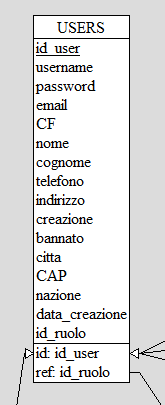
\includegraphics[]{UserLogico.png}
\end{center}

\item 
Generalizzazione dell’entità \textit{Eventi}: 
Analogamente, l’entità \textit{Eventi} era inizialmente strutturata come una generalizzazione totale ed esclusiva, comprendente i sottotipi \textit{Periodico} e \textit{Occasionale}, utilizzati per definire la natura dell'evento. Tuttavia, analizzando l’architettura del sistema, abbiamo ritenuto più efficiente eliminare la gerarchia e incorporare i sottotipi come attributi dell’entità principale \textit{Eventi}. Questa scelta ha permesso di mantenere la flessibilità nella classificazione degli eventi, riducendo al contempo la complessità del modello e facilitando la gestione delle informazioni relative agli eventi.
\begin{center}
    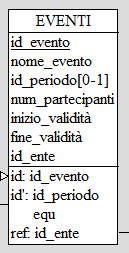
\includegraphics[]{EventiLogico.png}
\end{center}
\end{itemize}

\subsubsection{Chiavi esterne}
Vengono utilizzate, per semplicità, chiavi esterne con lo stesso nome della chiave primaria a cui fanno riferimento.




